\documentclass[11pt]{article}

\usepackage[margin=1in]{geometry}
\usepackage[T1]{fontenc}
\usepackage[utf8]{inputenc}
\usepackage{lmodern}
\usepackage{graphicx}
\usepackage{amsmath,amssymb,amsfonts}
\usepackage{textcomp}
\usepackage{xcolor}
\usepackage[hidelinks]{hyperref}
\usepackage{booktabs}
\usepackage{multirow}
\usepackage[numbers]{natbib}
\usepackage{tikz}
\usetikzlibrary{positioning, arrows.meta, fit, matrix, shapes.geometric}

\hyphenation{poly-chron-isa-tion combi-nato-rial nano-chat permu-tational}

\begin{document}

\title{\Large\textbf{Permutational Transformers --- Status Report}\\[2pt]
\large May 2026}

\author{Anatoly Starostin}
\date{}

\maketitle

\noindent\textbf{What this document is.}
This is a status report on the spiky permutational-transformer research line.
It is not a paper.
A paper requires a stable arc and a single message; we are still in the middle of an active exploration with multiple branches and many ideas that are interesting only in retrospect.
Instead the report fixes the present state in three layers: a brief introduction to the global task, a vague history of what we have already tried (sufficient to explain how we arrived at the current architecture), and a detailed description of the current model with its training setup, results, and diagnostics.
The closing section lists the open problems we are about to attack.
We intend to write similar reports on a regular cadence; subsequent ones will be deltas, much shorter than this one.


% ======================================================================
\section{Introduction}
\label{sec:intro}

\subsection{The global task}

Standard transformers~\cite{ref:vaswani} represent each token as a real-valued vector $\mathbf{x} \in \mathbb{R}^d$ and propagate information through linear projections and dot-product attention.
Information is carried in the \emph{magnitudes} of the vector components, and the basic operation is the multiply-accumulate.
This paradigm has scaled extraordinarily well, but it is not the only way to build an expressive sequence model.

The \emph{Spiking Manifesto}~\cite{ref:manifesto} proposes a different basis for computation, motivated by biology.
A sequence of $n$ distinguishable spikes admits $n!$ distinct timing patterns; a population of neurons can therefore encode information in the relative \emph{ordering} of its activities.
A magnitude-based vector in $\mathbb{R}^n$ at full floating-point precision nominally distinguishes vastly more states than $n!$, but that capacity is tightly coupled to fine numerical resolution: normalisation, quantisation, and additive noise collapse many states into equivalence classes.
The permutation capacity is, by contrast, robust --- it depends only on the relative ordering and is invariant to scaling, shifting, and any monotonic transformation of individual dimensions.
The corresponding computational primitive is a lookup table indexed by pairwise comparisons of the input, requiring only comparators and table reads --- no multiplications.

Our goal is to take this premise seriously and carry it through end-to-end into a working language model.
Concretely:
\begin{itemize}
\setlength{\itemsep}{2pt}
    \item \textbf{Encoding.} Replace magnitude-based embeddings with permutation embeddings: the carrier of information is the relative ordering of the components, not their numerical values.
    \item \textbf{Operations.} Replace most of the linear projections (dense matmuls) inside the transformer by multi-table lookup modules indexed by pairwise comparisons of the input.
\end{itemize}
The choice of attention mechanism (Kendall-$\tau$ via SDPA on dominance vectors, raw SDPA on LUT outputs, or other variants), the inter-block signal-flow structure (residual stream, concat-of-layer-outputs, rank-canonicalised stream), and which projections are most worth replacing first are open questions that we treat as exploration axes rather than fixed goals; different choices have appeared in the leading recipes at different times, and the current model in Section~\ref{sec:current} represents one specific resolution.

If this programme succeeds without losing accuracy versus a strong magnitude-based baseline, it potentially opens the door to very expressive but compact, highly compressed language models.
The expected source of that compression is the combinatorial structure itself: a comparator-based primitive operates on the order of the inputs rather than on their magnitudes, and the model that emerges should be able to use that combinatorial degree of freedom in a way that a magnitude-based architecture cannot.

\subsection{What this report covers}

The bulk of the report (Section~\ref{sec:current}) is a detailed description of the current operating point --- the hybrid soft / multi-alt LUT transformer that lives in the \texttt{exp265}--\texttt{exp267} cluster of our spiky tree.
Those three runs share an identical architecture and differ only in device batch size (8, 16, 32 respectively); we describe the architecture once and report results for all three.
It is not by every metric the best score we have ever obtained, but it is the cleanest expression of the architectural commitments above and the recipe from which the next set of experiments will branch.

Section~\ref{sec:evolution} sketches, in deliberately broad strokes, the chain of experiments that led here, so the design decisions in Section~\ref{sec:current} have a context.
Section~\ref{sec:future} lists the open problems we plan to attack next.

All code, configurations, and training logs referenced in this report live in the spiky repository,\footnote{\url{https://github.com/anatoli-starostin/spiky}} under \texttt{nanochat\_exps/} and (earlier) \texttt{transformer\_exps/}.


% ======================================================================
\section{Evolution of ideas (so far)}
\label{sec:evolution}

This section is deliberately compressed.
The actual record runs to several hundred experiments across two distinct phases (\texttt{transformer\_exps/} and \texttt{nanochat\_exps/} in the repository), and we make no attempt to enumerate them.
What we want to record is the chain of \emph{ideas} that survived long enough to shape the current architecture, so that the design choices in Section~\ref{sec:current} are not opaque.
This section is intentionally out of focus relative to that one.

\subsection{Phase 1 --- byte-level transformers (the \texttt{transformer\_exps/} era)}
\label{sec:evolution:bytelevel}

The first phase, several hundred experiments long, ran on byte-level FineWeb (vocabulary 257) with context lengths first 32 and later 128 tokens.
The vanilla transformer baseline under this protocol is val cross-entropy $\approx 1.36$ at 5M parameters (ctx-32) and $\approx 1.20$ at the same parameter count (ctx-128).
The ideas worth carrying forward from this phase, in roughly the order they emerged, are:
\begin{itemize}
\setlength{\itemsep}{2pt}
    \item \textbf{Reproduce-then-shrink.} A six-layer LUT transformer in the spirit of~\cite{ref:manifesto} --- each linear projection (Q, K, V, out-proj, FFN) replaced by a multi-head lookup module --- reaches a working loss but at $\sim$190M parameters. Most of phase~1 was about closing this parameter gap.
    \item \textbf{The \texttt{nap} / \texttt{tph} tradeoff.} A LUT module is parameterised by two numbers per head: \texttt{nap} (anchor pairs read per table $\Rightarrow$ table size $2^\text{nap}$) and \texttt{tph} (tables aggregated per head). At fixed budget, many small tables (\texttt{nap} $\sim$ 3--4) consistently outperform few large ones --- each table is a low-resolution router and superposing many covers input space better than refining a few.
    \item \textbf{Full-coverage anchor sampling.} Switching from random anchor-pair sampling to a policy that guarantees every $\binom{d}{2}$ input pair appears in at least one table gave a free $\sim$0.02 cross-entropy improvement and is the default in every LUT module since.
    \item \textbf{RankAttention via SDPA on dominance vectors.} The Kendall-$\tau$ rank correlation of two orderings $\mathbf{x}$, $\mathbf{y}$ equals the cosine similarity of their pairwise-sign signatures (the \emph{dominance vectors}, $\pm 1$ values indexed by ordered pairs). Permutational attention thus runs as standard scaled dot-product attention on dominance vectors --- no custom kernel needed. This trick was the dominant attention recipe for a long stretch; later we found that standard SDPA applied directly to the LUT-produced Q/K vectors (with QK-LayerNorm) can be at least as good and is simpler, so we now use both as a function of context.
    \item \textbf{LUT-emitted attention scores.} A more direct way to get permutational attention is to feed each ordered pair $(\mathbf{x}_i, \mathbf{x}_j)$, concatenated with a relational positional embedding $\mathbf{P}_{i-j}$, through a LUT that emits the attention score $s_{ij}$ directly. The pairwise concatenation $[\mathbf{x}_i \,|\, \mathbf{x}_j \,|\, \mathbf{P}_{i-j}]$ is the natural input form because it carries the full ordering information of the pair. The downside is computational: scores are produced for every $(i, j)$, so the LUT runs $T^2$ times per layer instead of $T$, with input dimensionality also doubled. The cost was prohibitive at the contexts we care about, which is why we ultimately stayed with the classic Q/K factorisation in the current model: a single LUT call per token producing per-head Q and K vectors that go into standard SDPA.
    \item \textbf{Move to ctx-128, mixed-\texttt{nap} budgeting.} Lengthening context to 128 reset the leaderboard. The choices that scaled were: small tables for Q/K (\texttt{nap} $\sim$ 5), big tables for out-proj and FFN (\texttt{nap} $\sim$ 10--12); QK LayerNorm before the attention dot product; and \emph{concatenation of per-layer outputs} as the unembedder input, replacing a residual sum. The natural combinatorial analogue of summation is concatenation, because summing two orderings is ill-defined --- the resulting order depends on magnitudes. The best ctx-128 LUT model in this era reached val $\approx 1.36$ at $\sim$300M parameters, matching the vanilla baseline at $\sim$60$\times$ the parameter cost.
    \item \textbf{BitPermutationLUT --- a parallel storage line.} A reparameterisation in which each LUT weight is a one-bit vote for a single pairwise dominance relation in the output space rather than a real-valued output component. With a custom straight-through Adam variant on bf16 latents, the bit-packed model matches the vanilla baseline on ctx-128 at $\sim$25\,MB of weights. This is the line that motivates the eventual hardware story: a forward pass made entirely of comparators, table reads, $\pm 1$ SDPA, and a small full-precision residue. A multi-bit intermediate ($K \in \{2, 4, 8\}$) is under study (\texttt{transformer\_exps/exp410--426}, $K=4$ currently the sweet spot).
\end{itemize}
Phase~1 is closed for active development; the current model and the future-work items in Section~\ref{sec:future} all live in the next phase.
The bit-quantisation line above is the major exception: it is a separate axis of investigation that we expect to fold back into the main recipe once the ranking-faithful trunk has stabilised.

\subsection{Phase 2 --- BPE on a real corpus (the \texttt{nanochat\_exps/} era)}
\label{sec:evolution:nanochat}

To run on a more realistic benchmark we ported the architecture to the nanochat tokeniser (BPE with $V = 32{,}768$) on the ClimbMix corpus, with a context of 512 tokens and an effective batch of 4096 tokens per gradient step.
This is the protocol used throughout the rest of the report.
The vanilla MinimalGPT under this protocol achieves val bits-per-byte (\texttt{bpb}) $1.626$ at 8K steps and $1.341$ at 48K steps.

The early portion of this phase repeated the ctx-128 design exploration on the new benchmark and recovered the same qualitative findings (full-coverage sampling, mixed-\texttt{nap} budgeting, Q/K LayerNorm, concat unembedder).
The 8K LUT bpb on the ranking-faithful trunk reached $\sim$1.74 in this period.
The work that followed moved this number down step by step.
The data-science findings worth recording, in chronological order:
\begin{itemize}
\setlength{\itemsep}{2pt}
    \item \textbf{Q/K capacity is the first lever, but bounded.} At embedding $E = 64$, increasing the Q/K-LUT \texttt{tph} (with everything else fixed) gave a clear single-knob improvement to $\sim$1.71 bpb at 8K. Sweeping \texttt{tph} further saturated --- attention scoring is essentially a binary discrimination task that cannot absorb arbitrary additional capacity.
    \item \textbf{Wider embedding ($E$).} Going from $E = 64$ to $E = 96$, with Q/K and V/out-proj capacities adjusted accordingly, brought the 8K bpb down to $\sim$1.63 and the 48K bpb to $\sim$1.51 --- the first sub-1.55 LUT result. Width matters more than per-pair vote density once the latter is past saturation.
    \item \textbf{Wider value channel ($d_v$).} Independently, increasing $d_v$ from 16 to 32 (and rebudgeting out-proj accordingly) gave another $\sim$0.01--0.02 bpb at 8K and $\sim$1.49 bpb at 48K. The value channel was the clearest secondary bottleneck.
    \item \textbf{Raw SDPA on LUT-emitted Q/K becomes competitive at $E = 96$.} A surprise from this stretch: at the wider embedding, replacing V2D-on-Q/K with QK-LayerNorm followed by raw SDPA on the LUT outputs is at least as good and sometimes better. The intuition we have for this is that at $E = 96$ the LUT outputs have enough numerical room for QK-norm to produce well-conditioned dot products without the dominance projection's sparsity. We have kept both attention variants in active use: the current model uses the raw-SDPA recipe.
    \item \textbf{Out-proj capacity should be front-loaded across layers.} A graded \texttt{tph} schedule (e.g. $[2048, 2048, 1024, 1024, 1024, 1024]$) consistently outperforms a flat schedule at the same total parameter count. This is consistent with the diagnostic finding in Section~\ref{sec:current} that early layers exploit their LUT capacity much more than late ones.
    \item \textbf{The TinyMultiHeadLut module: noise + two interchangeable backward modes.} The LUT module was rewritten to expose two backward paths (a soft routing over all $2^\text{nap}$ entries, and a multi-alt STE that routes only over $n_\text{alt}$ alternatives obtained by flipping the least-confident bits) plus a small training-time noise that flips the chosen anchor-pair sign at low-confidence comparisons. The soft path is more accurate but only affordable at small $\text{nap}$; the multi-alt path stays affordable at every $\text{nap}$. The hybrid choice (soft for small-$\text{nap}$ LUTs, multi-alt for large-$\text{nap}$ LUTs) is the architecture of Section~\ref{sec:current}; the noise is a small but stable regulariser ($\sim$$0.01$ bpb).
    \item \textbf{Bigger device batch.} Doubling the device batch from 8 to 16, with the effective batch held fixed at 4096 tokens, gave $-0.083$ bpb at 8K --- the largest single-knob improvement on this benchmark in months. The working hypothesis is that LUT training has uniquely sparse per-token gradients (each token visits only a handful of weight rows per LUT) so denser per-row statistics from bigger batches help the optimiser in a way that does not transfer to dense magnitude-based architectures.
\end{itemize}
The current 48K SOTA on the ranking-faithful trunk is $1.464$ bpb (TinyMultiHeadLut soft + noise, batch 8).
A faster recipe at 8K ($1.523$ bpb at hybrid + batch 16) is the cleanest current expression of the architectural commitments and is the object of Section~\ref{sec:current}.
A handful of recipes score $\sim$$0.02$ bpb better still on raw bpb but relax the ``purely ranking-coded'' commitment in the trunk and we treat them as off-strategy for this report.



% ======================================================================
\section{Current model: hybrid soft / multi-alt LUT transformer}
\label{sec:current}

The remainder of the report focuses on a single architecture, instantiated as three runs that differ only in device batch size: \texttt{exp265} (batch 8, val $1.613$ at 8K), \texttt{exp266} (batch 16, val $1.523$), and \texttt{exp267} (batch 32, val $\mathbf{1.450}$).
The architecture description (Sections~\ref{sec:current}.1--\ref{sec:current:flow}) applies to all three; results are reported jointly in Section~\ref{sec:current:results}.
The diagnostics in Section~\ref{sec:current:diag} were collected on the smaller-batch \texttt{exp265} checkpoint but transfer directly --- the per-LUT structure does not change with batch size.

\subsection{Architecture overview}

The model is a six-layer transformer with embedding dimension $E = 96$, six attention heads of dimensions $d_{qk} = 64$ and $d_v = 32$, and a context length of $T = 512$ tokens.
The token embedder is a standard $V \times E$ table with values uniform in $[-0.1, 0.1]$.
Each layer carries an additive learnable positional encoding $\mathbf{p}^{(\ell)} \in \mathbb{R}^{T \times E}$ (one per layer).
There are no inter-block residual connections; instead, the per-layer outputs are concatenated at the top of the stack and projected to vocabulary logits by a two-layer MLP unembedder (Section~\ref{sec:current:unembedder}).

Figure~\ref{fig:block} shows one block.
The block has three LUT modules (Q/K joint, V, and out-projection), one SDPA call, and a pair of conversions between materialised rankings and dominance vectors (the \emph{V2D} and \emph{D2V} layers) at the output boundary that keep the inter-block signal in ranking space.
Each LUT is implemented as a \texttt{TinyMultiHeadLut} (Section~\ref{sec:current:tinymhl}) configured according to the role it plays.

\begin{figure}[!t]
\centering
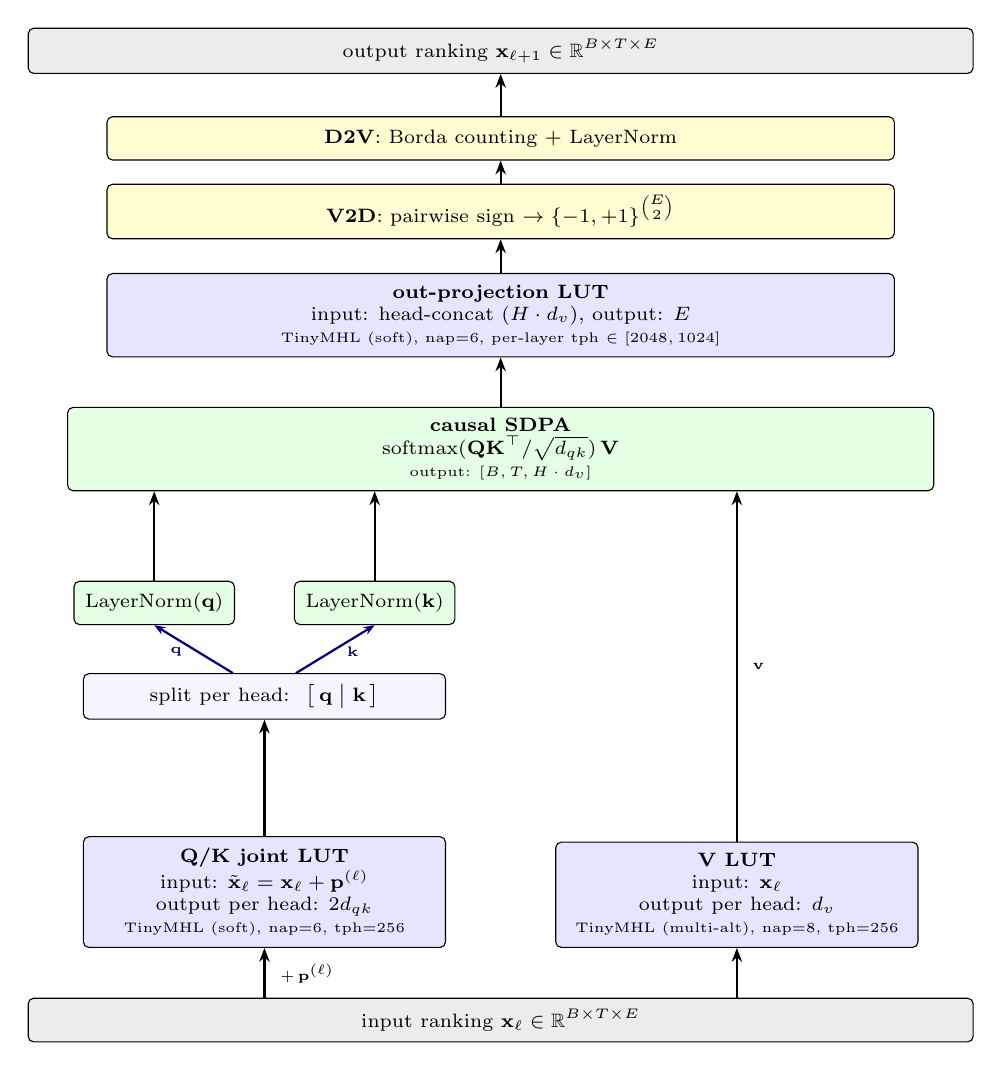
\begin{tikzpicture}[
    x=1cm, y=1cm,
    every node/.style={font=\scriptsize},
    box/.style={rectangle, draw, rounded corners=2pt, align=center, inner sep=4pt, fill=#1, minimum height=0.55cm},
    box/.default=blue!8,
    lut/.style={box=blue!10},
    op/.style={box=green!10},
    ln/.style={box=green!10, minimum width=1.8cm, minimum height=0.55cm},
    dom/.style={box=yellow!18, minimum height=0.55cm},
    edge/.style={box=gray!15, minimum width=12cm, minimum height=0.55cm},
    pass/.style={box=blue!4, minimum height=0.45cm},
    arr/.style={-{Stealth[length=5pt]}, thick},
    splitarr/.style={-{Stealth[length=4pt]}, thick, blue!50!black},
]
    % --- nodes (absolute coordinates, bottom-to-top) ---
    \node[edge, anchor=south] (xin) at (0, 0) {input ranking $\mathbf{x}_\ell \in \mathbb{R}^{B \times T \times E}$};

    % LUT modules: Q/K on left, V on right (well separated)
    \node[lut, minimum width=4.6cm, anchor=south] (qk) at (-3.0, 1.2)
        {\textbf{Q/K joint LUT}\\
         input: $\tilde{\mathbf{x}}_\ell = \mathbf{x}_\ell + \mathbf{p}^{(\ell)}$\\
         output per head: $2 d_{qk}$\\
         \tiny TinyMHL (soft), nap=6, tph=256};
    \node[lut, minimum width=4.6cm, anchor=south] (v) at (3.0, 1.2)
        {\textbf{V LUT}\\
         input: $\mathbf{x}_\ell$\\
         output per head: $d_v$\\
         \tiny TinyMHL (multi-alt), nap=8, tph=256};

    % Split node above the Q/K LUT
    \node[pass, minimum width=4.6cm, anchor=south] (split) at (-3.0, 4.1)
        {split per head: $\;\big[\, \mathbf{q}\;\big|\;\mathbf{k} \,\big]$};

    % LayerNorm(q) and LayerNorm(k) -- horizontally well separated
    \node[ln, anchor=south] (qn) at (-4.4, 5.3) {LayerNorm($\mathbf{q}$)};
    \node[ln, anchor=south] (kn) at (-1.6, 5.3) {LayerNorm($\mathbf{k}$)};

    % SDPA -- wide, well above the LN row (v feeds in directly from the V LUT)
    \node[op, minimum width=11cm, anchor=south] (sdpa) at (0, 7.0)
        {\textbf{causal SDPA}\\
         $\mathrm{softmax}(\mathbf{Q}\mathbf{K}^\top / \sqrt{d_{qk}})\,\mathbf{V}$\\
         \tiny output: $[B, T, H \cdot d_v]$};

    % Out-proj LUT
    \node[lut, minimum width=10cm, anchor=south] (op) at (0, 8.7)
        {\textbf{out-projection LUT}\\
         input: head-concat ($H \cdot d_v$), output: $E$\\
         \tiny TinyMHL (soft), nap=6, per-layer tph $\in [2048, 1024]$};

    % V2D / D2V
    \node[dom, minimum width=10cm, anchor=south] (v2d) at (0, 10.2)
        {\textbf{V2D}: pairwise sign $\to \{-1, +1\}^{\binom{E}{2}}$};
    \node[dom, minimum width=10cm, anchor=south] (d2v) at (0, 11.2)
        {\textbf{D2V}: Borda counting $+$ LayerNorm};

    % Output ranking
    \node[edge, anchor=south] (xout) at (0, 12.3)
        {output ranking $\mathbf{x}_{\ell+1} \in \mathbb{R}^{B \times T \times E}$};

    % --- arrows ---
    % input -> Q/K  (with positional add label)
    \draw[arr] (-3.0, 0.55) -- node[right=2pt, font=\tiny] {$+\,\mathbf{p}^{(\ell)}$} (qk.south);
    % input -> V
    \draw[arr] ( 3.0, 0.55) -- (v.south);

    % Q/K LUT -> split
    \draw[arr] (qk.north) -- (split.south);

    % split -> LayerNorm(q) and LayerNorm(k)
    % Diagonal "fork" from the [q|k] text in the split out to the two LayerNorm
    % boxes — so the visual reads as "q comes out of the q-half, k out of the
    % k-half, of the split node". Start points are slightly off split.north's
    % centre to land near the q and k characters in the rendered text.
    \draw[splitarr] ([xshift=-0.4cm]split.north) -- node[pos=0.45, left=2pt, font=\tiny] {$\mathbf{q}$} (qn.south);
    \draw[splitarr] ([xshift= 0.4cm]split.north) -- node[pos=0.45, right=2pt, font=\tiny] {$\mathbf{k}$} (kn.south);

    % LayerNorm(q), LayerNorm(k) feed into SDPA from below; v feeds in directly
    % from the V LUT top edge (single straight vertical line all the way up).
    \draw[arr] (qn.north) -- (-4.4, 7.0);
    \draw[arr] (kn.north) -- (-1.6, 7.0);
    \draw[arr] (v.north)  -- node[right=2pt, font=\tiny] {$\mathbf{v}$} ( 3.0, 7.0);

    % SDPA -> out-proj -> V2D -> D2V -> xout
    \draw[arr] (sdpa.north) -- (op.south);
    \draw[arr] (op.north)   -- (v2d.south);
    \draw[arr] (v2d.north)  -- (d2v.south);
    \draw[arr] (d2v.north)  -- (xout.south);
\end{tikzpicture}
\caption{One block of the current model, drawn bottom-to-top (input ranking $\mathbf{x}_\ell$ enters at the bottom, output ranking $\mathbf{x}_{\ell+1}$ leaves at the top). The Q/K joint LUT emits a per-head vector of width $2 d_{qk}$, which is split into a query $\mathbf{q}$ and a key $\mathbf{k}$ that pass through separate LayerNorms before SDPA. The V LUT emits per-head $\mathbf{v}$ directly into SDPA. The out-projection LUT output is then rank-canonicalised back to a ranking embedding by V2D (pairwise signs, $\binom{E}{2} = 4560$ values in $\{-1, +1\}$) followed by D2V (Borda counting and LayerNorm) before passing to the next block. There are no inter-block residual connections; per-layer outputs are concatenated at the top of the stack and projected to vocabulary logits (not shown).}
\label{fig:block}
\end{figure}

\subsection{The LUT primitive: TinyMultiHeadLut}
\label{sec:current:tinymhl}

A \texttt{TinyMultiHeadLut} module with $H$ heads, $T_h$ tables per head, anchor-pair count $n_c$, and output dimension $n_{\text{out}}$ implements
\begin{equation}
    \mathbf{y}_h \;=\; \sum_{t=1}^{T_h} W^{(h, t)}_{\, j_t(\mathbf{x})}, \qquad
    j_t(\mathbf{x}) \;=\; \sum_{k=1}^{n_c} \mathbf{1}[x_{a_{t,k}} > x_{b_{t,k}}] \cdot 2^{k-1},
    \label{eq:lut}
\end{equation}
where $W^{(h, t)} \in \mathbb{R}^{2^{n_c} \times n_{\text{out}}}$ is the per-table weight matrix and $\{(a_{t,k}, b_{t,k})\}$ are the anchor pairs sampled by the \texttt{CANONICAL\_FULL\_COVERAGE} policy (every distinct input pair appears in at least one table).
The module is parameterised by $H \cdot T_h \cdot 2^{n_c} \cdot n_{\text{out}}$ floating-point weights (fp32 in the current model).
Total weight count for the model is dominated by the out-projection LUTs (input dim $H \cdot d_v = 192$, $n_{\text{out}} = E = 96$, $\text{nap} = 6$, $\text{tph}$ between 1024 and 2048 per layer) and reaches $\sim$358M parameters.

The forward in~\eqref{eq:lut} is piecewise constant in $\mathbf{x}$.
Two backward modes are implemented:

\paragraph{Soft backward (used at $\text{nap}=6$: Q/K and out-proj).}
The forward of~\eqref{eq:lut} is unchanged --- it picks one entry per table by hard sign-bit packing.
The backward routes the gradient through \emph{all} $K = 2^{n_c}$ entries of each table via two stages, and is the more accurate of the two backward modes.
\begin{enumerate}
\setlength{\itemsep}{1pt}
    \item \textbf{Soft signs.} For each anchor-pair difference $\delta_{t,k} = x_{a_{t,k}} - x_{b_{t,k}}$, replace the hard $\mathrm{sign}(\delta_{t,k})$ used in the forward by the rational soft sign
    \begin{equation}
        p_{t,k} \;=\; \frac{\delta_{t,k}}{\tau_{\text{soft}} + |\delta_{t,k}|} \;\in\; (-1, +1),
    \end{equation}
    where $\tau_{\text{soft}}$ is a learnable per-LUT temperature initialised at $0.5$.
    Lower $\tau_{\text{soft}}$ approximates $\mathrm{sign}$ more sharply.
    \item \textbf{Soft routing.} For each candidate entry index $j \in \{0, \ldots, K - 1\}$ with bit pattern $\mathbf{b}_j \in \{-1, +1\}^{n_c}$, compute a match score $z_{t,j} = \mathbf{b}_j^\top \mathbf{p}_t$, then softmax along $j$ at a second learnable temperature $\tau_{\text{sel}}$ (also initialised at $0.5$),
    \begin{equation}
        \alpha_{t,j} \;=\; \mathrm{softmax}_j (z_{t,j} / \tau_{\text{sel}}).
    \end{equation}
    The bit-pattern reconstruction $\mathbf{b}_j$ is consistent with the forward's hard pick: the saved index is exactly $\arg\max_j z_{t,j}$ at fp32, so the chosen entry is also the modal entry of $\alpha_t$.
\end{enumerate}
The gradient flowing into table $t$ is then expanded as if the output had been the soft-routed combination $\sum_j \alpha_{t,j} W_{t,j}$ rather than the hard pick $W_{t, j^\star(\mathbf{x})}$.
Concretely, the gradient w.r.t.\ a table entry is the upstream gradient scaled by $\alpha_{t,j}$ (and accumulated at the chosen entry by an extra hard-scatter so the forward and backward agree in expectation), and the gradient w.r.t.\ the input flows back through $\partial p_{t,k} / \partial \delta_{t,k}$ and the anchor-pair indexing.
Both $\tau_{\text{soft}}$ and $\tau_{\text{sel}}$ receive their own gradients and tighten slightly during training.

The cost of accuracy is a per-table $[B \cdot T, K]$ intermediate that holds the soft routing weights; this is acceptable at $\text{nap}=6$ ($K = 64$) but becomes the dominant memory cost at $\text{nap}=8$ ($K = 256$), which is why the V LUT uses the cheaper multi-alt STE backward instead.

\paragraph{Multi-alt STE backward (used at $\text{nap}=8$: V).}
The gradient is computed only against the chosen entry plus the $n_{\text{alt}} = 3$ alternative entries obtained by flipping the least-confident bits.
Each alternative contributes via an inverse-$L_1$ uncertainty
\begin{equation}
    u(\delta) \;=\; \frac{0.5}{T + |\delta|},
\end{equation}
where $T$ is a per-LUT temperature, yielding a sparse top-$k$ scatter in place of the dense soft routing.
This makes the per-step memory bounded by $n_{\text{alt}}$ rather than by table size, which is what makes large-table modules trainable in practice.

\paragraph{Argmax-noise regularisation.}
In both modes, before the table index is computed, the chosen anchor-pair sign is flipped with probability $\varepsilon \approx 2 \cdot 10^{-3}$ at low-confidence comparisons (those with $|\delta_{t,k}|$ below a threshold), the parameter \texttt{argmax\_noise\_eps} in the LUT module.
The flip mask is saved so forward and backward see consistent indices.
This is a deliberately small perturbation; its effect is on the order of $-0.01$ bpb but stable across configurations.

\subsection{V2D and D2V: rank canonicalisation between blocks}
\label{sec:current:v2d}

The output of the out-projection LUT is a real-valued vector of dimension $E$.
By the time we cross the block boundary we want to have stripped its magnitude information so that the inter-block signal carries only the order of the components.
This is the role of the V2D and D2V layers.

\paragraph{V2D (vector to dominance).}
Given a real vector $\mathbf{y} \in \mathbb{R}^{E}$, the \emph{dominance vector} is the $\binom{E}{2}$-dimensional vector of pairwise sign comparisons:
\begin{equation}
    \mathrm{V2D}(\mathbf{y})_{ij} \;=\; \mathrm{sgn}(y_i - y_j), \qquad i < j.
    \label{eq:v2d}
\end{equation}
For $E = 96$ this is a $\binom{96}{2} = 4560$-dimensional vector with values in $\{-1, +1\}$.
$\mathrm{V2D}(\mathbf{y})$ depends on $\mathbf{y}$ only through its sort order $\sigma_\mathbf{y}$ and is invariant under any monotonic transformation of the components --- magnitudes are discarded.
The forward is piecewise constant in $\mathbf{y}$; in training we use the same rational soft sign as in the LUT backward,
\begin{equation}
    \mathrm{V2D}_{\text{soft}}(\mathbf{y})_{ij} \;=\; \frac{y_i - y_j}{\tau + |y_i - y_j|} \;\in\; (-1, +1),
\end{equation}
with a learnable temperature $\tau$ initialised at $0.1$, and a straight-through estimator that uses the hard $\mathrm{sgn}$ in the forward.

\paragraph{D2V (dominance to vector).}
The natural inverse of V2D is \emph{Borda counting}: the $i$-th coordinate of a ranking embedding can be reconstructed from the dominance vector as the number of components that $y_i$ beats minus the number it loses to,
\begin{equation}
    \mathrm{D2V}(\mathbf{d})_i \;=\; \frac{1}{E - 1} \sum_{j \neq i} \mathrm{sgn}(y_i - y_j),
    \label{eq:d2v}
\end{equation}
followed by a LayerNorm to put the result on a stable scale before the next block's LUT modules.
The Borda step recovers a length-$E$ vector whose component order matches the underlying ranking; the LayerNorm provides the modest scale stability the next layer's anchor-pair comparisons need at initialisation.

\paragraph{Why both directions.}
The out-projection LUT emits a real-valued vector of dimension $E$.
Its components carry both an order (the ranking we care about) and arbitrary magnitudes (artefacts of how many table entries summed to each component, and of the unconstrained scale of those entries).
We want only the order to propagate into the next block.
V2D extracts exactly that --- the dominance vector depends solely on the relative order of the components and is invariant to any monotonic rescaling --- and D2V then converts the dominance vector back into a length-$E$ ranking embedding so that the next block's Q/K/V LUTs receive the same shape they expect.
The composition $\mathrm{D2V} \circ \mathrm{V2D}$ is therefore the explicit ``magnitude stripper'' at the block boundary: it projects the out-projection's real-valued output onto the manifold of ``ranking embeddings'' (vectors whose information content is entirely in their sort order).
The LUTs themselves do not need this projection because their index function already depends only on signs of pairwise differences --- but the inter-block residual that V2D/D2V replaces would have carried magnitudes through, so the projection has to live somewhere on the per-block path.

\subsection{Per-block flow}
\label{sec:current:flow}

For an input $\mathbf{x}_\ell \in \mathbb{R}^{B \times T \times E}$, layer $\ell$ produces:
\begin{enumerate}
\setlength{\itemsep}{2pt}
    \item Add the layer's positional embedding: $\tilde{\mathbf{x}} = \mathbf{x}_\ell + \mathbf{p}^{(\ell)}$.
    \item \textbf{Q/K joint LUT.} A single \texttt{TinyMultiHeadLut} maps $\tilde{\mathbf{x}}$ to $2 d_{qk}$ outputs per head; the first $d_{qk}$ are interpreted as queries, the second $d_{qk}$ as keys. Configuration: $\text{nap}=6$, $\text{tph}=256$, soft backward.
    \item \textbf{QK-norm.} A LayerNorm on the $d_{qk}$ dimension is applied to Q and K separately (Qwen / Gemma style), without learnable scale.
    \item \textbf{V LUT.} A separate \texttt{TinyMultiHeadLut} maps $\mathbf{x}_\ell$ (no positional addition) to $d_v$ outputs per head. Configuration: $\text{nap}=8$, $\text{tph}=256$, multi-alt STE backward.
    \item \textbf{Causal SDPA.} Standard scaled dot-product attention $\text{softmax}(Q K^\top / \sqrt{d_{qk}}) V$ with a causal mask. The attention scale is the standard $1/\sqrt{d_{qk}}$ --- there is no learnable scale in the current configuration.
    \item \textbf{Out-projection LUT.} A third \texttt{TinyMultiHeadLut} maps the head-concatenated attention output (dimension $H \cdot d_v = 192$) back to the embedding dimension $E = 96$. Configuration: $\text{nap}=6$, $\text{tph}$ scheduled per-layer as $[2048, 2048, 1024, 1024, 1024, 1024]$ (front layers wider), soft backward. This is the largest module in the model.
    \item \textbf{V2D + D2V (rank canonicalisation).} The out-proj output is converted to its dominance vector (pairwise signs, $\pm 1$, $\binom{E}{2} = 4560$ coordinates), then back to a ranking embedding by Borda counting (sum each row of the dominance matrix) followed by LayerNorm. The out-V2D temperature is learnable, initialised at $0.1$. This step is what keeps the inter-block signal purely permutational --- the magnitude information that the LUT output's sum-of-tables structure would otherwise carry is discarded at this boundary, leaving only the ranking.
\end{enumerate}
Note that the LUT modules already ignore the magnitudes of their inputs (the index function in~\eqref{eq:lut} depends only on signs of pairwise differences), so the V2D/D2V step is the only place magnitudes would re-enter; the rank canonicalisation closes that gap.

There is, deliberately, \emph{no residual connection} of any kind inside the block.
A residual sum would mix a real-valued LUT output with the upstream ranking embedding and the resulting vector's order would depend on the relative magnitudes of the addends (the same magnitude leakage that the V2D/D2V step is designed to prevent).
Inter-layer information flow is therefore entirely through the layer-output concatenation at the top of the stack.

\subsection{Unembedder}
\label{sec:current:unembedder}

The per-layer block outputs $\mathbf{x}_1, \dots, \mathbf{x}_L$ are concatenated along the embedding axis into a $L \cdot E = 6 \cdot 96 = 576$-dimensional vector per token, which feeds a two-layer MLP unembedder
\begin{equation}
    \text{logits}(\mathbf{c}) \;=\; W_2 \cdot \text{GELU}\!\left( W_1 \cdot \text{LayerNorm}(\mathbf{c}) \right),
\end{equation}
with hidden dimension $4608$ and output dimension $V = 32{,}768$.
The unembedder is a standard fp32 dense module --- it is the only piece of the trunk that is not realised as a LUT.
This is a deliberate compromise: the unembedder converts a rank embedding into BPE-vocabulary logits, and a LUT-based version of that mapping (which we have explored in earlier ctx-128 work) is a separate axis of investigation that we are not yet folding into the main recipe.

\subsection{Training setup}

\paragraph{Data.}
nanochat tokeniser (BPE, $V = 32{,}768$) on the ClimbMix corpus.
Validation is bits-per-byte (\texttt{bpb}) on the canonical nanochat val split, evaluated every 200 steps over 10 batches.

\paragraph{Protocol.}
Context length $T = 512$.
Single forward/backward per optimiser step (no gradient accumulation): \texttt{exp265}, \texttt{exp266}, \texttt{exp267} use device batch $8$, $16$, $32$ respectively (effective batches $4096$, $8192$, $16{,}384$ tokens per step).
$8000$ steps total.
AdamW with $\text{lr} = 3 \cdot 10^{-4}$, $\beta = (0.9, 0.95)$, weight decay $0.1$ on $\ge 2$D parameters and $0$ on $<$2D parameters, $\epsilon = 10^{-8}$.
Cosine schedule with $10\%$ linear warm-up, decaying to $10\%$ of peak.

\paragraph{Hardware.}
Single NVIDIA H100 80\,GB.
Wall-clock time: $0.57$\,h for \texttt{exp265}, $1.15$\,h for \texttt{exp266}, $2.24$\,h for \texttt{exp267}.
Each batch doubling roughly doubles the step time.

\subsection{Results}
\label{sec:current:results}

\begin{table}[!t]
\caption{Headline results at the nanochat protocol. The vanilla baseline is MinimalGPT (a small GPT-2-style transformer, no LUTs) under the same protocol. The three LUT rows in the middle block are the same architecture (Sections~\ref{sec:current}.1--\ref{sec:current:flow}) at three different device batch sizes. The bottom row is a longer-horizon LUT run (\texttt{exp260}, 48K steps, batch 8): same architecture but with all-soft backward instead of the hybrid (the V LUT runs through the soft path too); the all-soft choice was what fit in memory at this longer horizon at the time the run was launched.}
\label{tab:current}
\centering
\begin{tabular}{lrrr}
\toprule
Model & Params & Steps & Val bpb \\
\midrule
Vanilla MinimalGPT (\texttt{exp001})                       & 23.4\,M   & 8K  & 1.626 \\
Vanilla MinimalGPT (\texttt{exp041})                       & 23.4\,M   & 48K & 1.341 \\
\midrule
LUT hybrid, batch 8  (\texttt{exp265})                     & 358\,M    & 8K  & 1.613 \\
LUT hybrid, batch 16 (\texttt{exp266})                     & 358\,M    & 8K  & 1.523 \\
\textbf{LUT hybrid, batch 32 (\texttt{exp267})}            & 358\,M    & 8K  & \textbf{1.450} \\
\midrule
LUT all-soft, batch 8 (\texttt{exp260})                    & 358\,M    & 48K & 1.464 \\
\bottomrule
\end{tabular}
\end{table}

Headline numbers are in Table~\ref{tab:current}.
At 8K steps and batch 8, the LUT model (\texttt{exp265}) already lands slightly below the vanilla MinimalGPT at the same compute budget; doubling the effective batch (\texttt{exp266}) gives $-0.090$ bpb, and doubling again (\texttt{exp267}) gives a further $-0.073$ bpb.
The cumulative effect of going from device batch $8$ to $32$ is $-0.163$ bpb at 8K, the largest stretch of single-knob improvement we have seen on this benchmark.
The longer-horizon LUT run \texttt{exp260} (48K steps, all-soft variant of the same architecture, batch $8$) reaches val bpb $1.464$ --- and \texttt{exp267} at 8K already passes it, at $\sim$$\frac{1}{6}$ of the training compute, so the headline finding is that batch scaling pays off enough to overtake six times the optimisation horizon.
The four short-horizon validation curves are in Figure~\ref{fig:val_three_way}; none of the LUT runs is plateauing at step 8000.

\begin{figure}[!t]
\centering
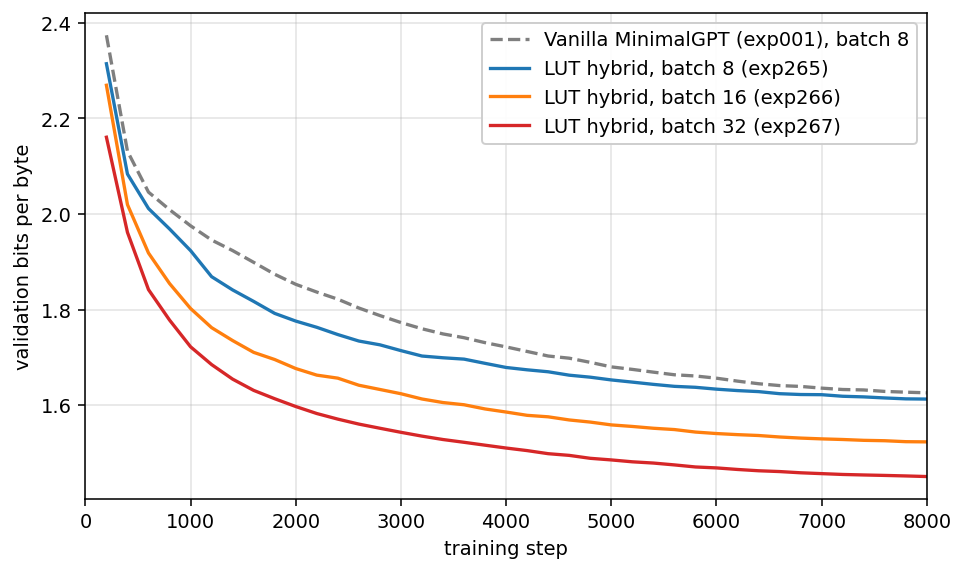
\includegraphics[width=0.92\linewidth]{figs/val_bpb_3way.png}
\caption{Validation bits per byte over training, all four runs at the same nanochat protocol (8000 optimiser steps each). The three LUT runs share an identical architecture and differ only in device batch size (8 / 16 / 32); each doubling shifts the whole curve downward and leaves it monotonically decreasing through step 8000. \texttt{exp267} at batch 32 is the current 8K SOTA.}
\label{fig:val_three_way}
\end{figure}

The picture at the longer 48K horizon is less favourable, and we want to be transparent about it.
The vanilla model and the LUT model start out at the same protocol but the LUT model's val bpb begins to flatten earlier: at $\sim$step 8000 the two curves cross, and from then on the vanilla model continues to improve while the LUT model trails by a slowly-widening margin.
By step 48000 the gap is $\sim$$0.12$ bpb (vanilla $1.341$, LUT $1.464$).
Figure~\ref{fig:val_three_way_48k} shows the two 48K runs; the early-training advantage of the LUT model is clearly visible, as is the long-horizon gap that opens after the crossover.
We do not yet know whether the gap is a fixed offset or whether vanilla would continue to pull ahead at even longer horizons.
The two natural attributions are (i) effective-batch starvation (\texttt{exp260} ran at device batch $8$, the largest that fit in memory at the time of launch; the new \texttt{exp265}--\texttt{exp267} short-horizon results suggest much of the gap closes when the batch is increased) and (ii) a residual capacity gap from the LUT primitive itself.
The 48K version of the \texttt{exp267} recipe (item~\textbf{1} of Section~\ref{sec:future}) is the experiment that will tell us which.

\begin{figure}[!t]
\centering
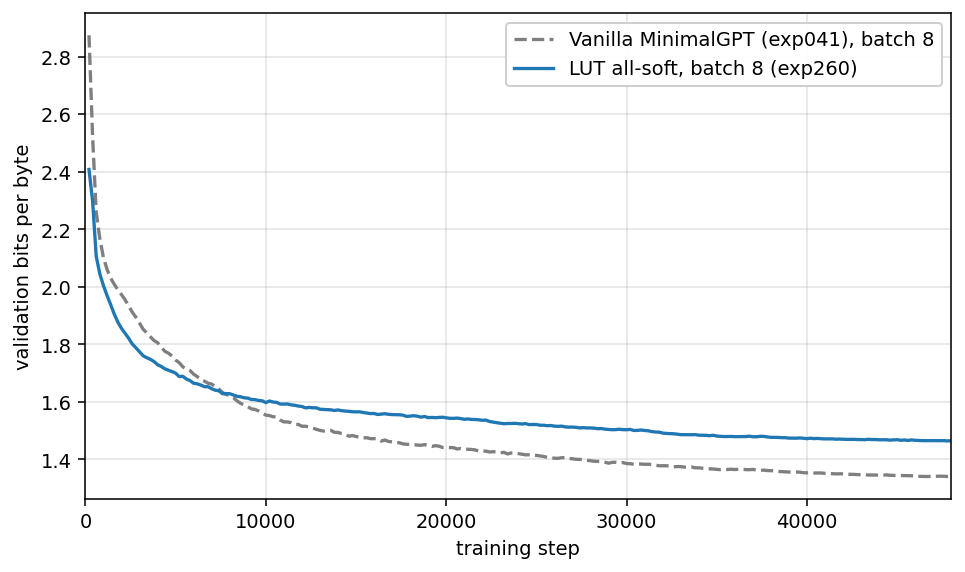
\includegraphics[width=0.92\linewidth]{figs/val_bpb_48k.png}
\caption{Long-horizon validation curves at 48000 steps. Both runs at device batch $8$. The LUT model leads early (the same effect visible in Figure~\ref{fig:val_three_way}) but is overtaken around step 8000; by step 48000 the vanilla baseline is ahead by $\sim$$0.12$ bpb. Whether this gap is a fixed offset or whether it would close with larger device batch (the new \texttt{exp265}--\texttt{exp267} short-horizon line suggests the latter) is open --- see Section~\ref{sec:future}, item~\textbf{1}.}
\label{fig:val_three_way_48k}
\end{figure}

\subsection{Bandwidth}
\label{sec:current:bandwidth}

The LUT model has $\sim$15$\times$ more parameters than the vanilla MinimalGPT (358M vs 23.4M), but the parameter count is misleading as a cost proxy.
The interesting per-step quantity is \emph{weight bandwidth}: how many weight values must be fetched from memory to compute one token's output.
For a dense matmul, the answer is the full weight tensor --- every weight contributes to every output position.
For a multi-table LUT with $K = 2^{n_c}$ entries per table, the answer is just $n_\text{heads} \cdot \text{tph} \cdot n_\text{out}$ values per token (the chosen entry per table); the other $K - 1$ entries per table are touched by other tokens but not by this one.
Per-token bandwidth thus scales with $\text{tph}$, not with the storage-bearing $K \cdot \text{tph}$.

Table~\ref{tab:bandwidth} works this out for the two models in fp32.

\begin{table}[!t]
\caption{Per-token weight reads (fp32 forward, no batch amortisation). Trunk reads include all per-layer projections summed over the six layers; for the LUT model these are LUT lookups, for the vanilla model they are dense matmul reads. Embedding reads are one row per layer per token.}
\label{tab:bandwidth}
\centering
\begin{tabular}{lrr}
\toprule
Component & Vanilla MinimalGPT & LUT model \\
\midrule
Trunk (all layers)      & $10{,}616{,}832$  ($\sim$42\,MB) & $\;\;2{,}260{,}992$  ($\sim$9\,MB) \\
Embedding lookups       & $\;\;\;\;\;\;\;\;\;\;\;\;768$  & $\;\;\;\;\;\;\;\;\;\;\;\;672$ \\
Unembedder              & $12{,}582{,}912$  ($\sim$50\,MB) & $153{,}650{,}304$  ($\sim$614\,MB) \\
\midrule
\textbf{Total per token} & $\mathbf{23{,}200{,}512}$  ($\sim$\textbf{93\,MB}) & $\mathbf{155{,}911{,}968}$  ($\sim$\textbf{624\,MB}) \\
\bottomrule
\end{tabular}
\end{table}

The trunk comparison is the headline number: the LUT trunk is $\sim$$5\times$ \emph{less} bandwidth than the vanilla trunk despite holding $\sim$$20\times$ more parameters --- exactly the LUT primitive's logarithmic capacity-vs-bandwidth payoff.
At a comparable trunk loss, the per-token weight bandwidth in the trunk is comparable to the vanilla model's total per-token bandwidth.

The total-model comparison goes the other way at present: the LUT model's MLP unembedder (a Linear($576 \to 4608$) followed by GELU and a Linear($4608 \to 32{,}768$), all fp32) is much wider than the vanilla model's tied lm\_head and reads $\sim$154M weights per token --- one matmul into the BPE vocabulary that no LUT primitive currently replaces.
Folding the unembedder into the LUT family --- so that its bandwidth scales with $\text{tph}$ instead of with the hidden width --- is future-work item~\textbf{3} below; once that gap is closed, the trunk's bandwidth advantage would carry through to the whole model.

\subsection{Diagnostics}
\label{sec:current:diag}

We ran two diagnostics on the trained \texttt{exp265} model (smaller batch but identical architecture, so the per-LUT structure transfers).
The questions:
\begin{enumerate}
\setlength{\itemsep}{2pt}
    \item \emph{Visit-frequency.} For each LUT, do the inputs route to diverse table entries, or concentrate in a small subset?
    \item \emph{Per-table SVD.} For each table, do the trained outputs span a high-dimensional subspace, or live in a low-dimensional one (the table is over-provisioned in $n_{\text{out}}$)?
\end{enumerate}
Together these answer ``is the LUT capacity actually exploited, or has it collapsed to a much smaller effective model?''.

The detailed numbers are in Table~\ref{tab:diag} and the takeaways are sharp:
\begin{itemize}
\setlength{\itemsep}{2pt}
    \item \textbf{L0--L2 use their capacity.} Visit entropy is near uniform ($H/\log K \ge 0.9$), no entries are unvisited, and the per-table SVD spans 50--65\% of full rank. This is what the manifesto picture implicitly claims: diverse inputs $\to$ diverse codes $\to$ non-trivial output subspace.
    \item \textbf{L3--L4 begin to specialise.} Visit entropy drops to $\sim$0.5--0.8, a small fraction of entries go unvisited, and the spectrum becomes peaky (top-4 singular values capturing 45--60\% of the Frobenius norm).
    \item \textbf{L5 has effectively collapsed.} Roughly $90\%$ of L5 entries are never visited on the validation set, and the visited entries' outputs live in a $\sim 7$-dimensional subspace out of 53 available. The last block is parameterised but not exercised.
\end{itemize}
This concentration is layer-specialised, not uniform.
A global ``the LUT model is over-provisioned'' or ``the LUT model is capacity-bound'' claim is misleading; the verdict depends on depth.
The actionable consequence is in Section~\ref{sec:future}: the last layer is the obvious target for capacity reduction (or for a different module structure such as hierarchical ferns), while early layers should not be touched.

\begin{table}[!t]
\caption{Per-LUT capacity-utilisation diagnostics on \texttt{exp265}. \texttt{util\_H} is the average normalised Shannon entropy of visit counts across tables (1.0 = uniform routing, 0 = single-entry); \texttt{unvis} is the average fraction of table entries that received zero visits over the validation set; \texttt{top10\%} is the average fraction of total visits captured by the 10\% most-visited entries (10\% if uniform); \texttt{r@90\%} is the smallest $k$ such that the top-$k$ singular values of the per-table weight matrix capture 90\% of its Frobenius norm. \texttt{full} is $\min(K, n_{\text{out}})$.}
\label{tab:diag}
\centering
\small
\begin{tabular}{lrrrrrr}
\toprule
LUT & $K$ & util\_H & unvis & top10\% & r@90\% / full & top-4 mass \\
\midrule
L0.qk\_joint  & 64  & 0.98 & 0.0\%  & 16\% & 36.5 / 64 & 28\% \\
L0.v\_lut     & 256 & 0.90 & 0.0\%  & 42\% & 20.5 / 32 & 38\% \\
L0.out\_proj  & 64  & 0.95 & 0.0\%  & 23\% & 32.6 / 64 & 28\% \\
\midrule
L1.qk\_joint  & 64  & 0.96 & 0.0\%  & 22\% & 18.3 / 64 & 44\% \\
L1.v\_lut     & 256 & 0.95 & 0.0\%  & 29\% & 17.1 / 32 & 63\% \\
L1.out\_proj  & 64  & 0.91 & 0.0\%  & 31\% & 35.0 / 64 & 24\% \\
\midrule
L2.qk\_joint  & 64  & 0.95 & 0.0\%  & 25\% & 18.2 / 64 & 45\% \\
L2.v\_lut     & 256 & 0.93 & 0.0\%  & 34\% & 19.9 / 32 & 57\% \\
L2.out\_proj  & 64  & 0.86 & 0.0\%  & 39\% & 35.7 / 64 & 23\% \\
\midrule
L3.qk\_joint  & 64  & 0.88 & 0.0\%  & 37\% & 18.9 / 64 & 47\% \\
L3.v\_lut     & 256 & 0.85 & 0.1\%  & 50\% & 19.8 / 32 & 57\% \\
L3.out\_proj  & 64  & 0.63 & 0.9\%  & 70\% & 34.7 / 64 & 29\% \\
\midrule
L4.qk\_joint  & 64  & 0.58 & 5.5\%  & 75\% & 14.4 / 64 & 59\% \\
L4.v\_lut     & 256 & 0.52 & 28.6\% & 89\% & 19.6 / 32 & 52\% \\
L4.out\_proj  & 64  & 0.29 & 48.2\% & 95\% & 18.3 / 64 & 45\% \\
\midrule
L5.qk\_joint  & 64  & 0.17 & 78.2\% & 99\% &  5.7 / 64 & 87\% \\
L5.v\_lut     & 256 & 0.12 & 93.2\% &100\% &  9.3 / 32 & 75\% \\
L5.out\_proj  & 64  & 0.05 & 94.8\% &100\% &  6.0 / 64 & 84\% \\
\bottomrule
\end{tabular}
\end{table}


% ======================================================================
\section{Open problems and future steps}
\label{sec:future}

This is the work the next set of experiments will tackle.
The list is intentionally short: each item is concrete enough to be a single experiment or a tight sweep.

\paragraph{1. Long-horizon batch scaling.}
Doubling the device batch from 8 to 16 to 32 has compounded better than expected ($-0.090$ then $-0.073$ bpb at 8K, see Section~\ref{sec:current:results}); \texttt{exp267} at batch 32 already beats the on-strategy 48K SOTA at $\sim$$\frac{1}{6}$ of the optimisation horizon.
The natural next step is the same recipe at 48K, which should push the on-strategy SOTA well below the current $1.464$ bpb of \texttt{exp260}.
There is also no sign of saturation: the validation curves are still monotonically decreasing at step 8000 for every batch size, and a further batch doubling (to $64$) is the obvious sub-experiment if memory permits.
This is the highest-priority next experiment.

\paragraph{2. Cut the last-layer capacity.}
Table~\ref{tab:diag} shows that L5's tables are visited by $\sim$10\% of inputs and produce outputs in a $\sim$7-dimensional subspace --- it is parameterised but not exercised.
The simplest test is an \texttt{out\_tph\_per\_layer} schedule that slashes the last two layers (e.g.\ $[2048, 2048, 1024, 1024, 512, 256]$) and checks that bpb is preserved.
A more aggressive variant cuts the last block entirely.
Either way the goal is a smaller model at the same loss.

\paragraph{3. LUT-based unembedder.}
Section~\ref{sec:current:bandwidth} (Table~\ref{tab:bandwidth}) shows that the LUT trunk has $\sim$$5\times$ less per-token bandwidth than the vanilla trunk despite holding $\sim$$20\times$ more parameters --- but the LUT model's dense MLP unembedder (Linear $576 \to 4608$ then $4608 \to V$) reads $\sim$154M weights per token and ends up dominating total bandwidth.
Replacing the unembedder with a LUT-family module (or at least replacing its wide hidden Linear with one) would let the trunk's bandwidth advantage carry through to the whole model.
The unembedder has its own design constraint that the trunk does not --- its output dimension is the BPE vocabulary $V = 32{,}768$, much larger than any per-layer dimension in the trunk --- so the choice of LUT primitive for this position is not obvious; this dovetails with item~\textbf{5} below.

\paragraph{4. Storage: the MultiBitPermutationLUT line.}
The current model is fp32 throughout (except the bf16 latents inside the soft backward).
The PermutationLUT line of work (the recent \texttt{exp410--426} batch in \texttt{transformer\_exps/}) shows that the same architecture compresses cleanly to $K \in \{1, 2, 4, 8\}$ bits per weight via a midrise quantiser, with $K=4$ emerging as the sweet spot.
Folding that quantisation into the current ranking-faithful trunk is a natural next step; the engineering cost is the optimiser-side bookkeeping (the bit-LUT optimiser variant of straight-through Adam) and is well understood.

\paragraph{5. Other ranking processors.}
Lookup tables are one specific learned mapping from rank-encoded inputs to outputs, but they are not the only one --- the broader question is what general family of \emph{ranking processors} is most expressive at fixed budget, and the multi-table sum~\eqref{eq:lut} is just one point in that space.
Within the LUT family, hierarchical lookups (random forests, hierarchical \emph{FERNS}) are an immediate next variant, motivated by the late-layer ``mode collapse'' visible in Table~\ref{tab:diag}: a coarse stage that picks a mode and a fine stage that refines within it would match what the visit distribution shows is happening anyway.
Other directions in the same neighbourhood include factored / low-rank LUTs, key-value retrieval over a small learned codebook, and randomised tabular substitutes for narrow projections.
At the more exotic end one can imagine entirely non-tabular processors --- for example, a small spiking reservoir whose readout is trained to mimic a target rank-to-rank map, or other dynamical systems on the permutation group --- which would be much harder to train but much closer to the biological substrate that motivated the project in the first place.
It would be interesting to explore other options.


% ======================================================================
\section*{Acknowledgement}

We are grateful to Yuval Aviel for the visit-frequency / SVD diagnostic that produced Table~\ref{tab:diag} and shaped the future-work direction on layer-specific capacity.


% ======================================================================
\begin{thebibliography}{99}

\bibitem{ref:manifesto}
E.~Izhikevich, ``Spiking Manifesto,'' arXiv:2512.11843, Dec.~2025.

\bibitem{ref:vaswani}
A.~Vaswani, N.~Shazeer, N.~Parmar, J.~Uszkoreit, L.~Jones, A.~N.~Gomez, \L.~Kaiser, and I.~Polosukhin,
``Attention is all you need,'' in \emph{Proc.\ NeurIPS}, 2017.

\bibitem{ref:fineweb}
G.~Penedo et al., ``The FineWeb Datasets: Decanting the Web for the Finest Text Data at Scale,'' arXiv:2406.17557, 2024.

\bibitem{ref:adam}
D.~P.~Kingma and J.~Ba, ``Adam: A method for stochastic optimization,'' in \emph{Proc.\ ICLR}, 2015.

\end{thebibliography}

\end{document}
